\chapter{The AFM}

\section{Overview}

Atomic force microscopy (AFM) is a technique that allows the 3D characterization of many types of samples (conductive, insulators, inorganic, organic, biological, etc.) and operates in air or liquid phase. Given its versatility, AFM can be coupled with other techniques by using specialized hardware and types of probes (e.g., scanning thermal microscopy, Kelvin probe force microscopy, infrared nanospectroscopy, etc). AFM, including various hyphenated techniques, permit analysis in various fields, such as polymer chemistry and physics, surface chemistry, cell biology, semiconductor science, and metrology.

The AFM topography results from the dilation of the sample shape, probe shape, and tip-sample-substrate interactions. An AFM image is commonly referred to as a 3D representation, although it is more referred to as a 2.5D reconstruction. The topography is a mapping of the heights given by a 2D array of numbers, which corresponds to the deflection of the cantilever as the tip scans the sample surface. Therefore, a not complete 3D reconstruction of the exposed surface is obtained, albeit limited by the tip geometry. In fact, it does not consider the portion of the sample in contact with the substrate. \cite{ribotta3}

The core of an AFM is its head, where the cantilever is located, which has the tip at its end. To scan the sample we drag a probe, known as the AFM tip, across it and register its elevation. Whenever the tip encounters an obstacle, it tries to match its height and to overcome it. The change of height is registered by the AFM using a laser-mirror system that converts the height displacement into an electric signal as shown in Fig. \ref{fig:AFM}.

\newpage

\begin{figure}[h]
    \centering
    % schema_afm
    \includegraphics[width=.6\textwidth]{./immagini/_power_afm4.png}
    \caption{AFM working principle}
    \label{fig:AFM}
\end{figure}

\section{Operational modes}

The AFM can operate in 3 different ways: contact mode, non-contact mode and tapping, based on the force region the AFM operates as shown in Fig. \ref{fig:AFM_modes_a}:
\begin{itemize}
    \item Contact mode: the deflection of the cantilever, proportional to the tip-sample
    interaction forces, provides sample topography.
    \item Non-contact mode: the vibration of cantilever at its resonance frequency is modified in amplitude and phase, due the interaction forces. To generate the images obtained in this work, the amplitude modulation was used, which gives not only topographic information, but also provides a feedback to keep the tip-sample distance constant (See Fig. \ref{fig:AFM_modes_b}).
    \item Tapping: the oscillation of the cantilever allows the tip to contact the sample cyclically, hence the force required to detach the tip from the sample is applied.
\end{itemize}

\newpage

\begin{figure}[h]
    \centering
    % schema_afm
    \includegraphics[width=0.95\textwidth]{./immagini/_power_afm3.png}
    \caption{Force region of operability}
    \label{fig:AFM_modes_a}
\end{figure}

\begin{figure}[h]
    \centering
    % schema_afm
    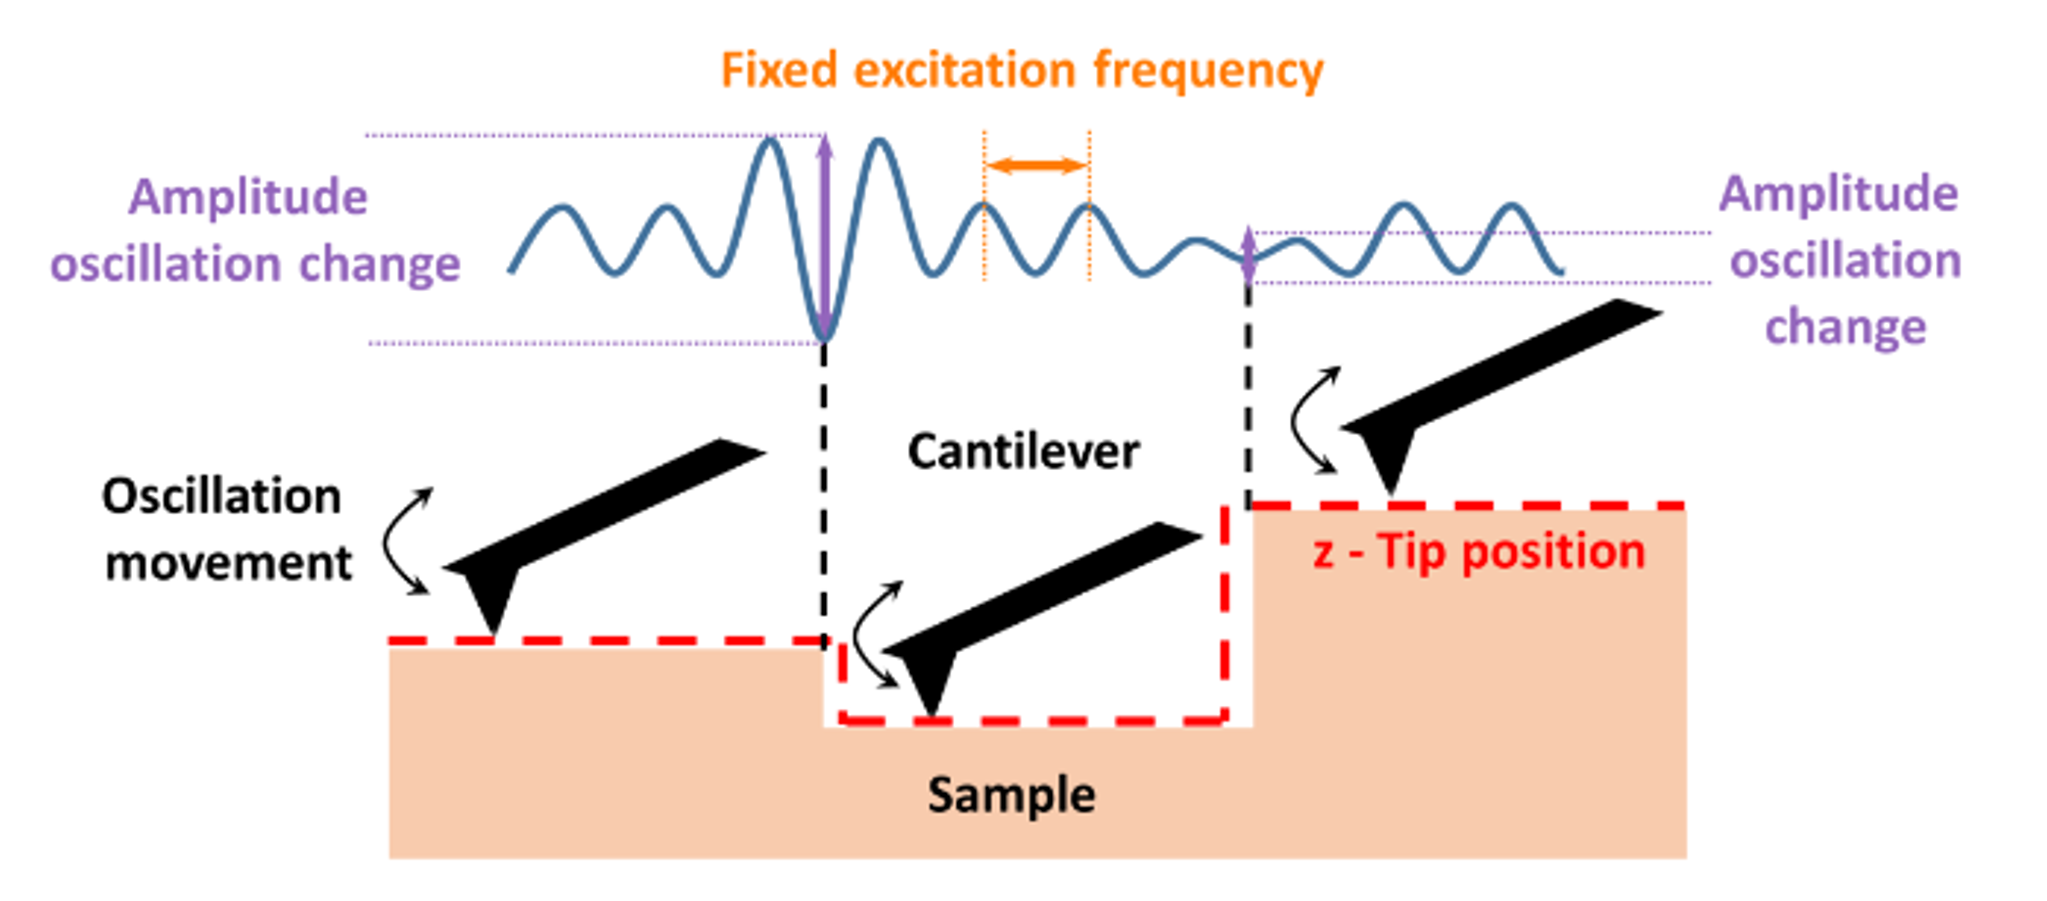
\includegraphics[width=.8\textwidth]{./immagini/non_contact_mode.png}
    \caption{Sketch of an AFM cantilever operating in non-contact mode (amplitude modulation) \cite{immagine_luigi}}
    \label{fig:AFM_modes_b}
\end{figure}

% \begin{figure}[ht]
%     \centering
%     \begin{subfigure}[b]{0.48\textwidth}
%         % forces
%         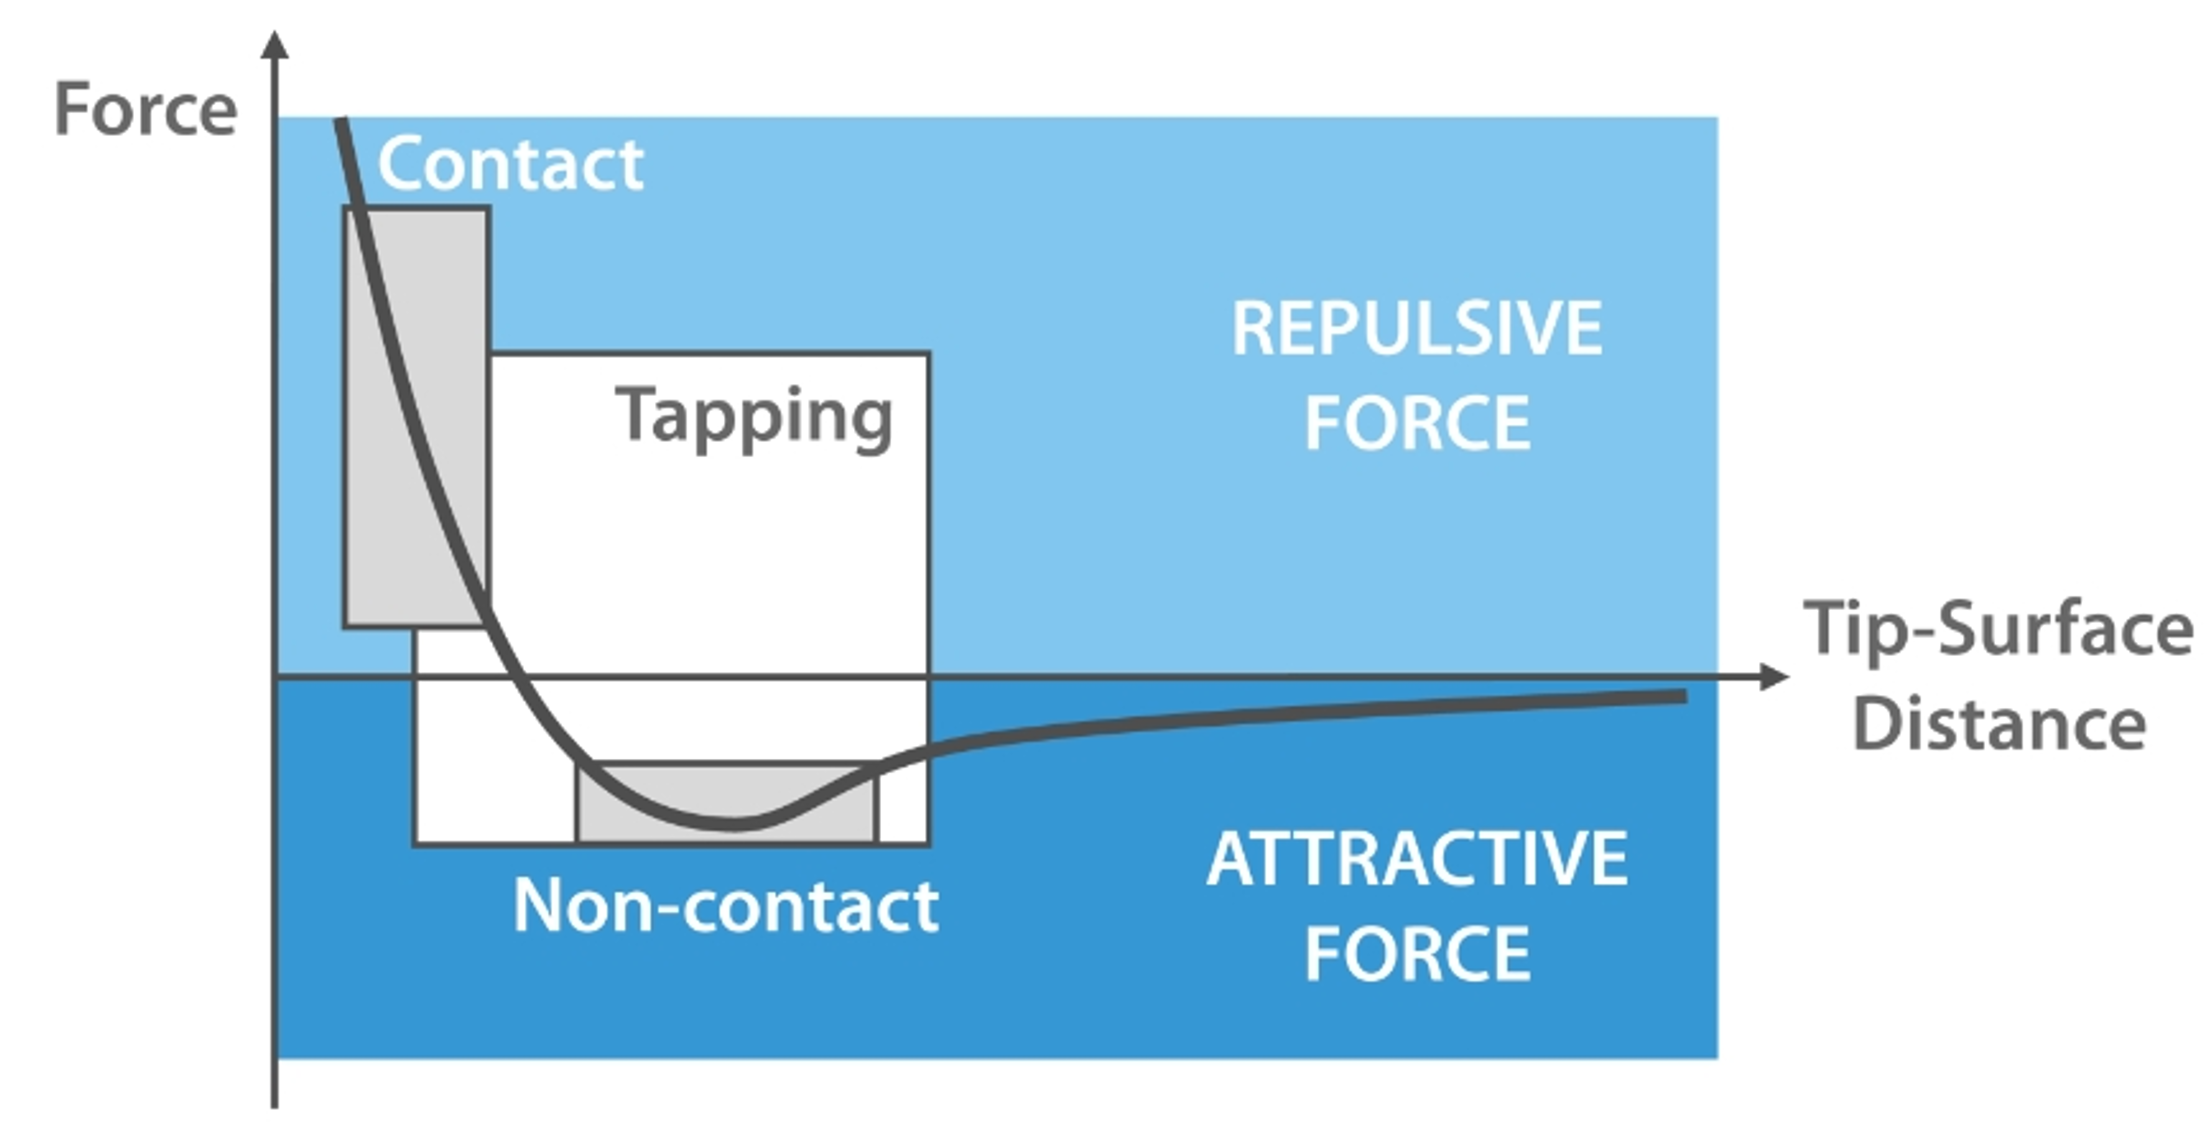
\includegraphics[width=.98\textwidth]{./immagini/forces.png}
%         \caption{}
%         \label{fig:AFM_modes_a}
%     \end{subfigure}
%     \hfill
%     \begin{subfigure}[b]{0.48\textwidth}
%         % non_contact_mode
%         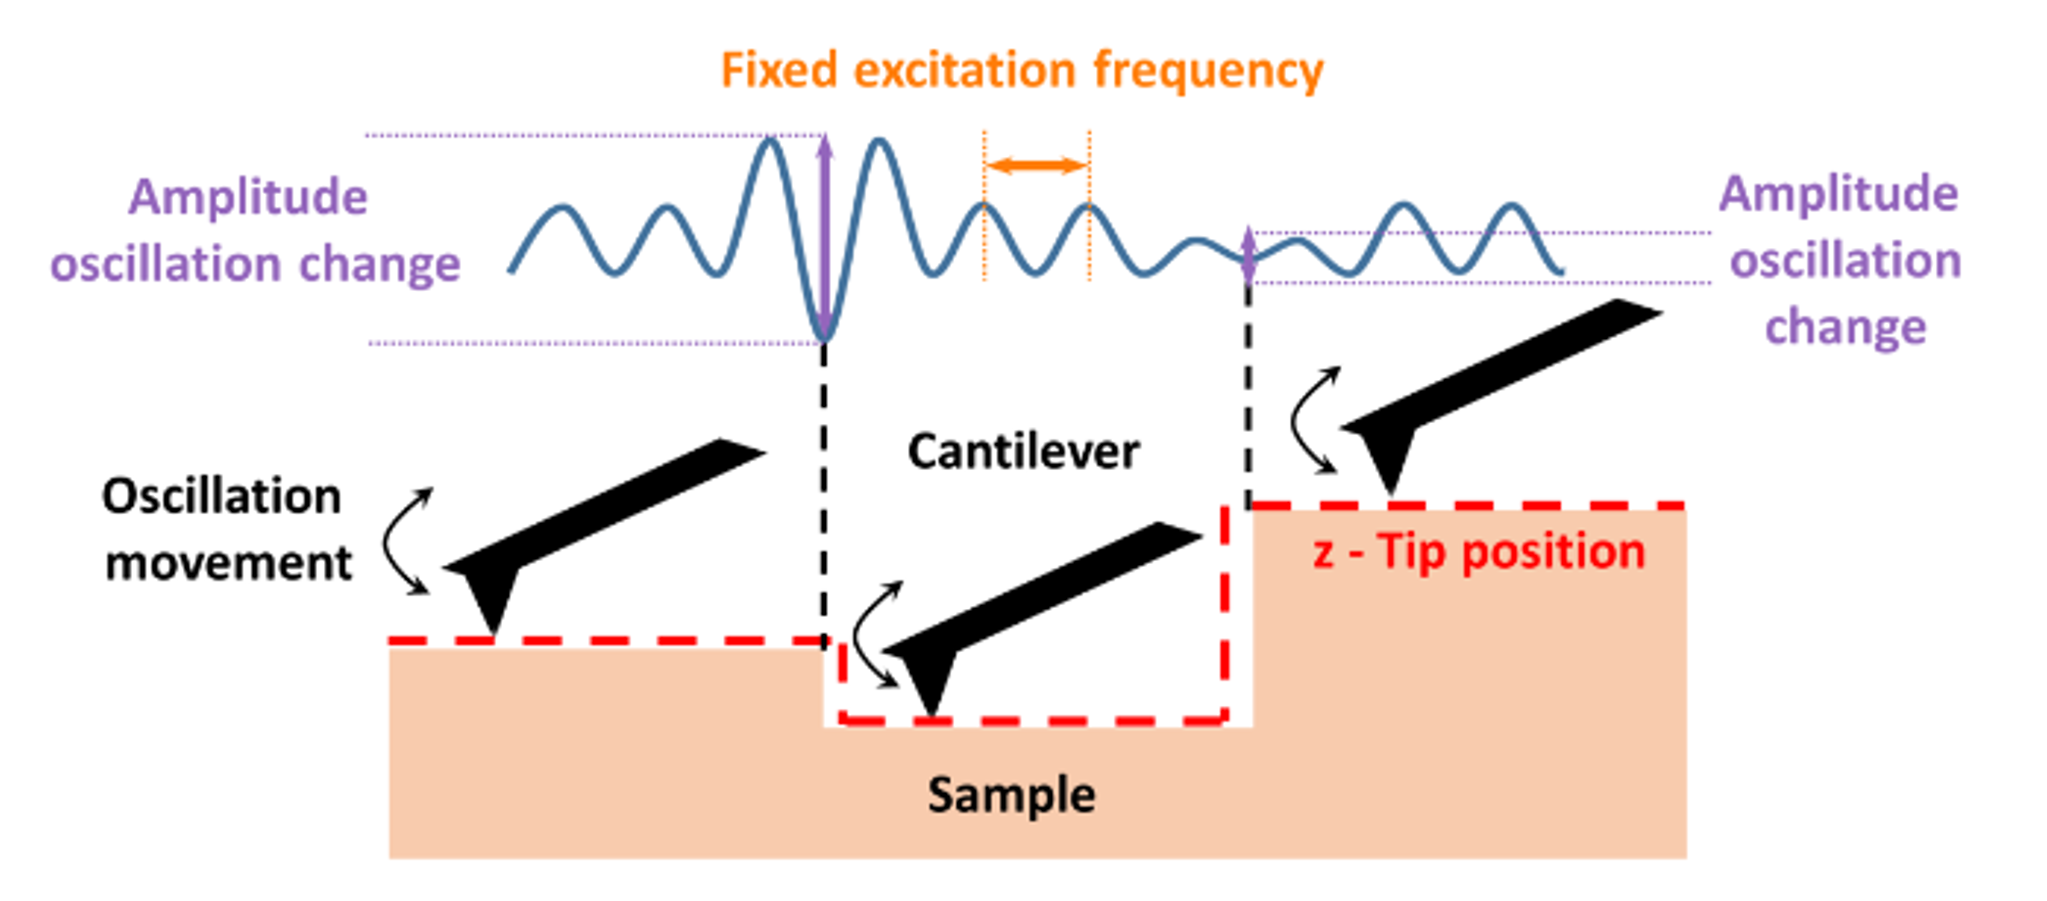
\includegraphics[width=.98\textwidth]{./immagini/non_contact_mode.png}
%         \caption{}
%         \label{fig:AFM_modes_b}
%     \end{subfigure}
%     \caption{a) Force region of operability b) Sketch of an AFM cantilever operating in non-contact mode (amplitude modulation) \cite{immagine_luigi}}
%     \label{fig:AFM_modes}
% \end{figure}

In this work, we focus on improving the lateral resolution of the AFM image, by removing the interference of the tip from the topography. It is known that the tip has an actual physical size, that deteriorates the lateral resolution. In fact, the quality of the lateral resolution is given by the tip-sample interaction and by the pixel size. Tip-sample and tip-substrate interactions refer to elasticity, whereas sample-substrate deformation refers to plasticity. 
    
The specific AFM used to generate these images is a custom made metrologic AFM, where everything except the head (obtained from Bruker) was designed and built at INRiM labs. This was achieved by building around the AFM a set of 3 interferometers, one along each axis, which guarantees the direct traceability to the SI (The International System of Units). The used tip $\mu$Masch (NSC-AlBS-14) \cite{ribotta3} works in non-contact mode.
